%\title{LaTeX Portrait Poster Template}
%%%%%%%%%%%%%%%%%%%%%%%%%%%%%%%%%%%%%%%%%
% a0poster Portrait Poster
% LaTeX Template
% Version 1.0 (22/06/13)
%
% The a0poster class was created by:
% Gerlinde Kettl and Matthias Weiser (tex@kettl.de)
% 
% Adapter by Jens Buysse for Hogeschool Gent
% This template has been downloaded from:
% http://www.LaTeXTemplates.com
%
% License:
% CC BY-NC-SA 3.0 (http://creativecommons.org/licenses/by-nc-sa/3.0/)
%
%%%%%%%%%%%%%%%%%%%%%%%%%%%%%%%%%%%%%%%%%

%----------------------------------------------------------------------------------------
%	PACKAGES AND OTHER DOCUMENT CONFIGURATIONS
%----------------------------------------------------------------------------------------

\documentclass[a0,portrait]{a0poster}

\usepackage{multicol} % This is so we can have multiple columns of text side-by-side
\columnsep=100pt % This is the amount of white space between the columns in the poster
\columnseprule=3pt % This is the thickness of the black line between the columns in the poster

\usepackage[svgnames]{xcolor} % Specify colors by their 'svgnames', for a full list of all colors available see here: http://www.latextemplates.com/svgnames-colors

\usepackage{times} % Use the times font
%\usepackage{palatino} % Uncomment to use the Palatino font

\usepackage{graphicx} % Required for including images
\graphicspath{{figures/}} % Location of the graphics files
\usepackage{booktabs} % Top and bottom rules for table
\usepackage[font=small,labelfont=bf]{caption} % Required for specifying captions to tables and figures
\usepackage{amsfonts, amsmath, amsthm, amssymb} % For math fonts, symbols and environments
\usepackage{wrapfig} % Allows wrapping text around tables and figures
\usepackage[export]{adjustbox}

\begin{document}

%----------------------------------------------------------------------------------------
%	POSTER HEADER 
%----------------------------------------------------------------------------------------

% The header is divided into two boxes:
% The first is 75% wide and houses the title, subtitle, names, university/organization and contact information
% The second is 25% wide and houses a logo for your university/organization or a photo of you
% The widths of these boxes can be easily edited to accommodate your content as you see fit

\begin{minipage}[t]{0.75\linewidth}
\VeryHuge \color{HoGentAccent1} \textbf{Opschalen van een autodeelsysteem: optimalisatie van het reservatiealgoritme} \color{Black}\\ % Title
\huge \textbf{Tim Alenus, Rik Bellens, Wim Goedertier}\\[0.5cm] % Author(s)
\huge Hogeschool Gent, Valentin Vaerwyckweg 1, 9000 Gent\\[0.4cm] % University/organization
\Large \texttt{tim.alenus.y9731@student.hogent.be} \\
\end{minipage}
%
\begin{minipage}[t]{0.25\linewidth}

\includegraphics[width=13cm,right]{figures/HOGENT_Logo_Pos_rgb.png} 

\end{minipage}

\vspace{1cm} % A bit of extra whitespace between the header and poster content

%----------------------------------------------------------------------------------------

\begin{multicols}{2} % This is how many columns your poster will be broken into, a portrait poster is generally split into 2 columns

%----------------------------------------------------------------------------------------
%	ABSTRACT
%----------------------------------------------------------------------------------------

\color{HoGentAccent1} % Navy color for the abstract

\begin{abstract}
Dit onderzoek onderzoekt één van de mogelijke optimalisaties van het reservatiesysteem van een autodeler: de gebruiker niet zelf een auto laten kiezen tijdens het reserveren, maar een auto laten toewijzen door een algoritme zodat de beschikbare auto's optimaal worden ingevuld. Het toewijzingprobleem wordt opgelost aan de hand van een Constraint Satisfaction Problem (CSP). Op basis van een dataset van historische reservaties werden simulaties uitgevoerd telkens met een verschillend aantal reservaties en een verschillend aantal beschikbare auto's. Voor elke simulatie werd de toewijzing van de auto's aan de reservaties éénmaal willekeurig gedaan en éénmaal aan de hand van de oplossing van het corresponderende CSP. Voor zowel de willekeurige toewijzing als voor de toewijzing met behulp van een CSP werd het service level, gedefinieerd als het percentage van reservaties dat kan doorgaan, en de actieve tijd per auto berekend. Uit de resultaten van de simulaties kan afgeleid worden dat er maar kleine winstmarges te boeken zijn voor het service level en de actieve tijd per auto door gebruik te maken van een CSP. Naarmate het systeem drukker en complexer wordt doordat het meer reservaties dient te verwerken en meer auto's bevat, lijken de winstmarges te groeien. Door het gebruik van een niet-performant algoritme om het CSP op te lossen was dit onderzoek echter gelimiteerd om de complexiteit van de gesimuleerde systemen op te drijven. Een vervolg op dit onderzoek zou een meer geavanceerd algoritme kunnen gebruiken om het CSP op te lossen.
\end{abstract}
%----------------------------------------------------------------------------------------
%	INTRODUCTION
%----------------------------------------------------------------------------------------

\color{HoGentAccent1} 
\section*{Introductie}
\color{black}
\color{black}
Partago is een coöperatie die elektrische auto's beschikbaar stelt aan haar coöperanten om te delen. Om dit mogelijk te maken heeft Partago een eigen software platform ontwikkeld. Deze software wil voldoen aan de specifieke noden die ontstaan wanneer een groep van gebruikers onderling elektrische auto's wil delen. Het Partago platform bestaat uit een applicatie voor de smartphone en een managementtool om de operationele processen die gepaard gaan met het delen van een elektrische vloot te ondersteunen.
Partago-auto's staan in zones. Momenteel maakt een gebruiker een reservatie voor een specifieke auto of kiest hij voor spontaan gebruik van een specifieke auto. Hierdoor wordt er echter niet optimaal gebruik gemaakt van de verschillende auto's die beschikbaar zijn binnen één zone. Een voorbeeld: Karel, Joachim en Clara willen allen gebruik maken van een auto in de zone Brugse Poort. De Brugse Poort is de thuislocatie van twee auto's: auto1 en auto2. Karel maakt een reservatie voor auto1 van 10h tot 12h. Joachim maakt een reservatie voor auto2 van 14h-17h. Clara wil ook gebruik maken van een Partago-auto. Zij zou de auto nodig hebben van 11h tot 16h. Er is echter geen enkele auto beschikbaar gedurende die tijdsspanne. Moesten Karel en Joachim echter beide gebruik maken van auto1 zou Clara nog perfect gebruik kunnen maken van auto2. Het systeem dwingt dit echter op geen enkele manier af. Een alternatieve mogelijkheid om het reserveringssysteem op te stellen zou zijn dat de gebruikers geen specifieke auto reserveren, maar een zone. Zo zou het systeem voor de zone reservaties ontvangen van Karel voor 10h tot 12h, van Joachim voor 14h tot 17h en van Clara voor 11h tot 16h. Het systeem zou dan zelf een toewijzing kunnen doen om zoveel mogelijk gebruikers tevreden te stellen.
\paragraph{Onderzoeksvraag}
Het onderzoek beschreven in deze bachelorproef wil een antwoord vinden op de vraag of het service level en de gebruiksduur van de auto's van Partago zou stijgen wanneer de gebruikers geen specifieke auto's reserveren, maar enkel een zone. Nadien wordt dan door het systeem een toewijzing gedaan wie welke fysieke auto krijgt. Deze onderzoeksvraag vormt de kern van het onderzoek. We definiëren het service level als het percentage van aangevraagde ritten dat daadwerkelijk ook kan doorgaan omdat er minstens nog één auto vrij is.
%----------------------------------------------------------------------------------------
%	GEOLOGY
%----------------------------------------------------------------------------------------

\color{Black} % DarkSlateGray color for the rest of the content
\color{HoGentAccent1} 
\section*{Experimenten}
\color{black}
Met een zelf ontwikkelde simulatietool werden simulaties uitgevoerd voor een verschillend aantal reservaties en een verschillend aantal beschikbare auto's. De gesimuleerde periode was telkens een periode van 4 weken. De reservaties gebruikt in een simulatie komen uit een dataset van historische reservaties gedaan op het systeem van Partago tussen 1 januari 2019 en 30 juni 2019. De reservaties in een simulatie gedragen zich dus als reëele Partago reservaties. Uit de dataset van historische reservaties wordt een dataset van 4 weken samengesteld voor de simulatie. Het aantal reservaties hangt af van de te simuleren druktegraad. De reservaties worden willekeurig gekozen uit de dataset van historische gegevens en gemapt op 1 van de 4 weken in de simulatie met behoudt van dag van de week. Omdat de reservaties willekeurig gekozen worden uit de historische reservaties zullen de reservaties in de simulatie niet in chronologische volgorde staan. In het reëele systeem komen reservaties immers ook niet chronologisch toe. Een reservatie voor 16h 's middags komt niet per se toe na een reservatie voor 8h 's ochtends. Voor de gegenereerde dataset in de simulatie wordt dan telkens een eenvoudige toewijzing gedaan en een toewijzing met behulp van het oplossen van de corresponderende CSP's. Voor volgende sets van parameters werden simulaties uitgevoerd: 
\begin{center}
	\label{tab:parameters}
	\begin{tabular}{ | l | l | l | p{3cm} |}
		\hline
		Aantal reservaties & Aantal auto's & Druktegraad & Aantal weken \\ \hline
		108 & 3 & 9 reservaties/week/auto & 4 \\ \hline
		180 & 5 & 9 reservaties/week/auto & 4 \\ \hline
		180 & 3 & 15 reservaties/week/auto & 4 \\ \hline
		300 & 5 & 15 reservaties/week/auto & 4 \\ \hline
		360 & 3 & 30 reservaties/week/auto & 4 \\ \hline
		600 & 5 & 30 reservaties/week/auto & 4 \\ \hline
	\end{tabular}
\end{center} 

\color{HoGentAccent1} 
\section*{Resultaten}
\color{black}


\begin{center}\vspace{1cm}
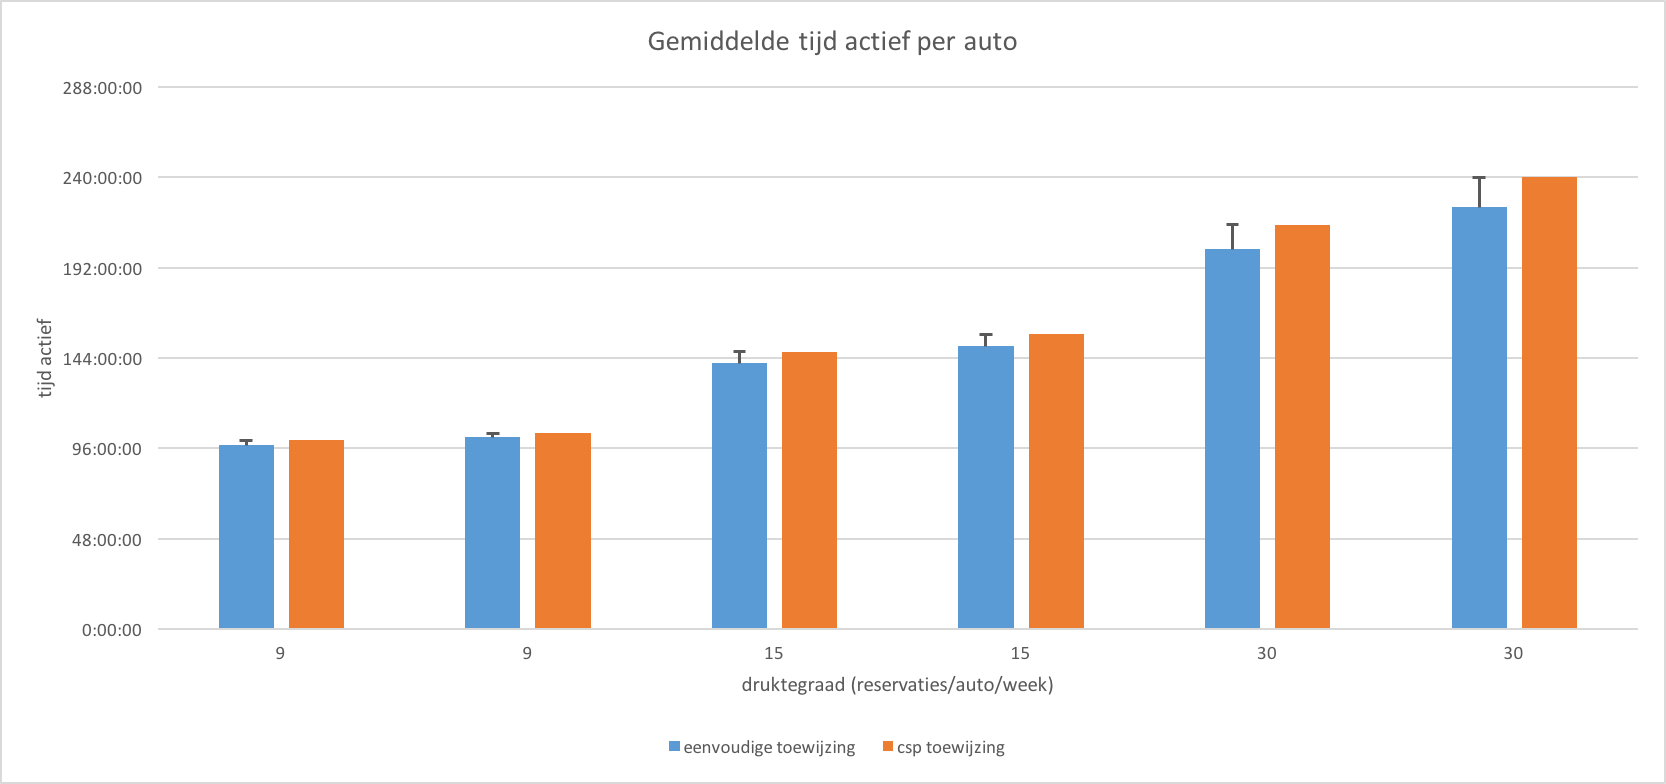
\includegraphics[width=1.0\linewidth]{grafiek-gemiddelde-tijd-actief-per-auto.png}
\label{grafiek1}
\captionof{figure}{\color{HoGentAccent5} Grafiek van de gemiddelde tijd actief per auto per druktegraad.}
\end{center}\vspace{1cm}
\begin{center}\vspace{1cm}
	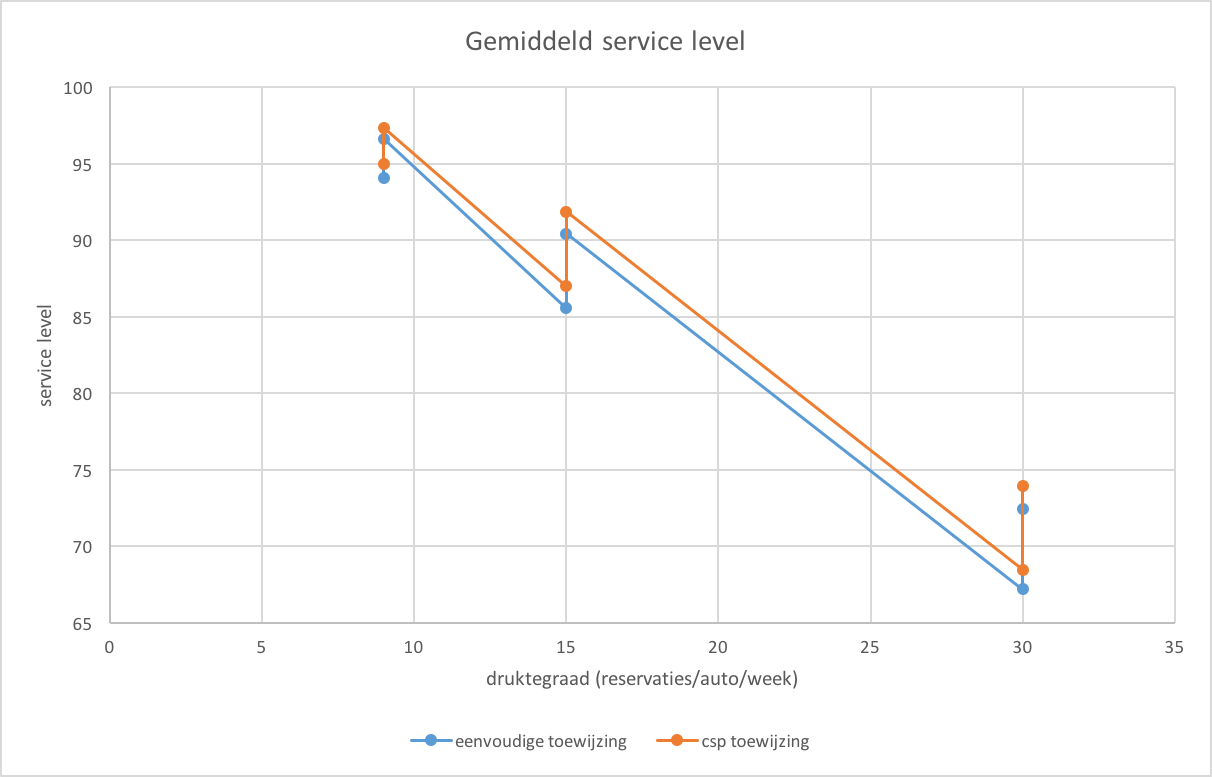
\includegraphics[width=1.0\linewidth]{grafiek-gemiddeld-service-level.png}
	\label{grafiek2}
	\captionof{figure}{\color{HoGentAccent5} Grafiek van het gemiddelde service level}
\end{center}\vspace{1cm}
Beide figuren vatten de resultaten van de simulaties goed samen. Figuur  \ref{grafiek1} toont de gemiddelde tijd dat een auto actief was. Blauw is met de eenvoudige toewijzing, oranje met de toewijzing met behulp van CSP's. Voor alle simulaties was de tijd actief met het toewijzingsalgoritme hoger in vergelijking met de eenvoudige toewijzing. Figuur \ref{grafiek2} vertoont gelijke resultaten. Het service level voor de toewijzing met CSP's ligt steeds hoger dan de eenvoudige toewijzing.

%------------------------------------------------



\color{HoGentAccent1} 
\section*{Conclusies}
\color{black}
De verbeteringen voor zowel het service level als voor de actieve tijd van een auto zijn relatief klein. Voor het service level werd over alle simulaties heen een gemiddelde verbetering van 1,2\% waargenomen. Naarmate het systeem complexer wordt met meer reservaties en meer auto's lijkt de winstmarge van de toewijzing met CSP's te groeien ten opzichte van de eenvoudige toewijzing. Dit wordt ook weergegeven in figuur \ref{grafiek1}. De simulaties met hogere drukte graad, rechts in de figuur, vertonen een groter verschil tussen blauw (de eenvoudige toewijzing) en oranje (de toewijzing met CSP's)
%----------------------------------------------------------------------------------------
%	FORTHCOMING RESEARCH
%----------------------------------------------------------------------------------------
\color{HoGentAccent1} 
\section*{Toekomstig onderzoek}
\color{black}
Een grote beperking van dit onderzoek is het relatief kleine aantal datapunten die gebruikt zijn. De originele opzet met het uitvoeren van simulaties met zelf geschreven code was om een groot aantal datapunten te kunnen genereren voor een meer diverse set van parameters van de simulaties. De simulatietool gebruikt in dit onderzoek is geschreven in Dart, net zoals de rest van het systeem van Partago. Voor de programmeertaal Dart bestaat er slechts 1 bibliotheek voor het oplossen van CSP's. Deze software bibliotheek is een zeer eenvoudige en niet-performante implementatie zonder gebruik van de verschillende optimalisatiemogelijkheden zoals heuristieken. Hierdoor liep de rekentijd exponentieel op naarmate het probleem complexer werd. De rekentijd voor de uitgevoerde simulaties in dit onderzoek is nu reeds meer dan 100 uur. Verder onderzoek zou dit onderzoek kunnen herhalen, maar om het CSP op te lossen gebruik maken van meer performante manieren zoals de OptaPlanner gerefereerd in het onderzoeksvoorstel van dit onderzoek. 

%----------------------------------------------------------------------------------------

\end{multicols}
\end{document}